\chapter{Implementation Details}

\section{SECube Firmware}
SEcube is the smallest reconfigurable silicon combining three main cores in a single-chip design. Low-power ARM Cortex-M4 processor, a flexible and fast Field-Programmable-Gate-Array (FPGA), and an EAL5+ certified Security Controller (SmartCard) are embedded in an extremely compact package. This makes it a unique security environment where each function can be optimised, executed, and verified on its proper hardware device \cite{secubesite}.
The SECube device has been the selected platform that allowed to build the entire Secure Password Manager application on top of it. This is due to, as introduced before, to all the security feature that are intrinsically implemented in the chip itself, both from the point of view of the hardware and software.\newline\newline
In fact, one of the most important security enabling technology is the 3D SiP (System-in-package); the device consists of a number of integrated circuit, each one built on top of the others and enclosed into a single package.\newline\newline
Not only the system is secure from the hardware point of view, that is a necessary condition in order to develop a secure software, but the already present firmware includes some high level functions to generate a secure channel only after the authentication.

Authentication is performed from both parties, in which not only the firmware checks the authenticity of the Host but, the also the Host can do the same. This is possible thanks to a pre-shared key that is stored in the device at the very first initialization of the device itself. A custom C program, after the firmware has been uploaded, allows to setup the master password for the Secure Password Manager. This implies that the password used to authenticate the Host application is configurable only once, allowing to simplify the entire authentication process for the new feature without reducing the security. Further consideration about the user usability and the security aspects are available at Section \ref{sec:weakness}.\newline\newline
The authentication is performed using a challenge-based authentication from both sides using a MAC (Message Authentication Code) implementation called Hash-based Message Authentication Code (HMAC), that uses a secret and an hash algorithm to verify the solution of the challenge. The challenge is created thanks to the internal TRNG (True Random Noise Generator), that is an hardware included in the chip that generates a true random sequence of bits. Once the challenge has been sent to the party to be authenticated and solved, the solution is read back and checked. If it corresponds to the expected one, the party is authenticated and the channel create. A small possible weakness study is available at \ref{sec:weakness}.

\subsection{Flash memory management}
Data are saved in the internal Flash memory, by using a C structure define as follow: 
\begin{lstlisting}[style=CStyle]
	typedef struct se3_flash_pass_ {
		uint32_t id;
		uint16_t host_size;
		uint16_t user_size;
		uint16_t pass_size;
		uint8_t* host;
		uint8_t* user;
		uint8_t* pass;
	} se3_flash_pass;
\end{lstlisting}
The Image \ref{fig:sepassrecord} shows a simplified representation of all the used field.
\begin{figure}[H]
	\centering
	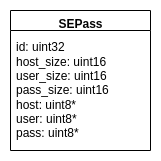
\includegraphics[width=0.2\linewidth]{images/firmware/sepass_record}
	\caption{SECube firmware password record represented using ER database schema}
	\label{fig:sepassrecord}
\end{figure}

Internally, some checks has been performed in order to inhibit the user to enter twice the same password record. This check is based on evaluating if the couple hostname and username is already present, and it is performed when the user modifies or creates a new password record. This has been made on purpose, since it has been assumed that a user can have two accounts for the same site and, even if wrong, he or she can use the same password for both of them. This has been implemented using a support method available in \texttt{se3\_pass.c} file, refer to Code \ref{code_sepass_equal}.

More precisely, data are stored in the flash memory using as few bits as possible to make the implementation able to store a large number of passwords, accordingly to the following table:
\begin{table}[H]
	\begin{tabular}{ c c l }
		\textbf{Field name} & \textbf{Number of bytes} & \textbf{Description}\\ 
		\hline
		\texttt{id} & 4 & Id to univocally identify a password, using 32 bits\\ 
		\hline
		\texttt{host\_size} & 2 & Number of character is the \texttt{host} \\  
		\hline
		\texttt{user\_size} & 2 &  Number of character is the \texttt{user} \\  
		\hline
		\texttt{pass\_size} & 2 &  Number of character is the \texttt{pass} \\  
		\hline
		\texttt{host} & \texttt{host\_size} & Hostname of the password record \\  
		\hline
		\texttt{user} & \texttt{user\_size} & Username of the password record\\  
		\hline
		\texttt{pass} & \texttt{pass\_size} & Plain text of the password record\\  
		\hline
	\end{tabular}
\caption{Flash memory for storing a Password record}
\label{tab:flashmem_pass}
\end{table}

The adopted solution allows to use 4 bytes for the id, and 2 bytes for the hostname, username and password length. The length of the other parameters are dependent on the previous three. This implies that at maximum $2^{16} = 65536$ characters can be used, but the system is able to reduce at minimum the occupied size, since the stored bits are not fixed.\newline\newline
Data into the Flash memory are stored as defined by the C structure shown at Table \ref{tab:flashmem_pass}. Since the internal embedded Flash memory is limited, a possible attack could rely on the fact that creating few record with the hostname, username and password length set to the maximum could fill up the space. This corresponds a DoS (Denial of Service) attack, making the system not more fully usable, by saturating the internal memory.

A solution to this problem could be to limit the number of characters of the hostname, username and password itself to a maximum value. The problem is that even in this case, if the user has an access to the device and it is logged in, he or she will be able to saturate the memory, independently from the dimension of each field. For this reason and for possible future improvements based on using the unused bits in the fields, 2 bytes have been reserved for each field.


\subsection{Code implementation}

The entire solution has been developed using the C language and everything has been built on top of the already present firmware.

Besides all the adaptations to the code that has been necessary to the Secure Password Manager to work correctly, everything is based on two C files under the ``\textit{SEcube USBStick Firmware/Project/Src/Device}" directory:
\begin{itemize}
	\item \texttt{se3\_sepass.c}
	\item \texttt{se3\_pass.c}
\end{itemize}

A coarse grain classification can be done on the level of data manipulation that the functions inside each one of the two files contains. In the case of \texttt{se3\_sepass.c}, functions are much more command oriented, allowing to perform rather complex operation by calling directly a function from the just received command. On the other hand, \texttt{se3\_pass.c} includes the functions for directly managing the Flash memory and abstract over some redundant operations, like the fetch from the storage. 


\subsubsection{Command dispatcher}
The \texttt{se3\_dispatcher\_core.c} file contains the code implementation for managing the custom commands that are necessary to provide to the Host application, in order to manage the passwords.\newline\newline
In order to add the five different commands needed to manage all the Secure Password Manager features (add, delete, modify, search and password generation), a custom command, with id 13 has been added. The five methods have been added by exploiting the sub-command management; part of the command payload is used to identify the id of the method to call. The implementation and management is available at Code \ref{code_command_disp}.

\begin{lstlisting}[style=CStyle,caption="Code for searching if password record is already present", label=code_command_disp,breaklines=true]
	uint16_t sepassword_manager_utilities(uint16_t req_size, const uint8_t* req, uint16_t* resp_size, uint8_t* resp)
	{
		uint16_t operation; // the type of operation to be executed
		memcpy((void*)&(operation), (void*)req, 2);
		se3_flash_it it = { .addr = NULL};
		if(!login_struct.y)
		{
			return SE3_ERR_ACCESS;
		}
	
		se3_flash_it_init(&it);
		it.addr = NULL;
		switch (operation)
		{
			case SE3_SEPASS_OP_ADD:
			return add_new_password(req_size, req+2, resp_size, resp);
			break;
			case SE3_SEPASS_OP_MODIFY:
			return modify_password(req_size, req+2, resp_size, resp);
			break;
			case SE3_SEPASS_OP_DELETE:
			return delete_password(req_size, req+2, resp_size, resp);
			break;
			case SE3_SEPASS_OP_GET_BY_ID:
			return get_password_by_id(req_size, req+2, resp_size, resp);
			break;
			case SE3_SEPASS_OP_GETALL:
			return get_all_passwords(req_size, req+2, resp_size, resp);
			break;
			case SE3_SEPASS_OP_GENERATE_RANDOM:
			return generate_random_password(req_size, req+2, resp_size, resp);
			break;
			default:
			SE3_TRACE(("[sepassword_utilities] invalid operation\n"));
			return SE3_ERR_PARAMS;
		}
		return SE3_OK;
	}	
\end{lstlisting}



\subsubsection{se3\_pass.c}
As already introduced before, the \texttt{se3\_pass.c} contains all the low level operations with the Flash memory. The most important available methods are the following:
\begin{itemize}
	\item \texttt{se3\_pass\_find}: given a password id, returns true if that id used
	\item \texttt{se3\_pass\_new}: given a password record, create a new password record in the Flash memory
	\item \texttt{se3\_pass\_read}: read from the Flash memory the password information of a single password
	\item \texttt{se3\_pass\_equal}: return true if there is a password with the same hostname and same username. The implementation is available at \ref{code_sepass_equal}
\end{itemize}

\begin{lstlisting}[style=CStyle,caption="Code for searching if password record is already present", label=code_sepass_equal,breaklines=true]
	bool se3_pass_equal(se3_flash_pass* password, se3_flash_it* it)
	{
		bool areEquals = false;
		se3_flash_pass tmp;
		se3_flash_it_init(it);
		
		while (se3_flash_it_next(it) && !areEquals)
		{
			if (it->type == SE3_TYPE_PASS)
			{
				se3_pass_read(it, &tmp);
				
				if (tmp.id == password->id || (is_str_eq(tmp.host, tmp.host_size, password->host, password->host_size) && is_str_eq(tmp.user, tmp.user_size, password->user, password->user_size)))
				{
					areEquals = true;
				}
				
				if(tmp.host != NULL) {free(tmp.host);}
				if(tmp.user != NULL) {free(tmp.user);}
				if(tmp.pass != NULL) {free(tmp.pass);}
			}
		}
		
		return areEquals;
	}
\end{lstlisting}



\subsubsection{se3\_sepass.c}
\label{sec:se3_sepass.c}
Differently form the \texttt{se3\_pass.c} file, the \texttt{se3\_sepass.c} contains high level oriented functions that are directly called by the sub-command command dispatcher for the password manager.\newline\newline
The available methods are the following:
\begin{itemize}
	\item \texttt{add\_new\_password}: used to generate a new password. The parameters such as the hostname, the username and the password are extracted from the command parameters checked against the current state of the Flash. More precisely, besides the consistency checks are performed before parsing the parameters, the pair hostname and username is searched into the memory, if not present the new password record is created. One important aspect is that the id of the new password is generated outside the device, and it is duty of the Host application to provide a valid value. This has been done in order to increase the flexibility of the solution and to allow the Host to use any kind on enumeration.
	\item \texttt{modify\_password}: similarly form the \texttt{add\_new\_password} function, the parameters are read and checked. Only if the id is present, the previous record is deleted and replaced by the new one with all the correct information.
	\item \texttt{delete\_password}: this simply deletes the password record by a given id
	\item \texttt{get\_all\_passwords}: return a list of all the passwords. It is also possible to filter by username or hostname
	\item \texttt{get\_password\_by\_id}: given an id, the password record is returned
	\item \texttt{generate\_random\_password}: given the length and the set of characters that must be used, a random password is generated using the internal TRNG.
\end{itemize}

The password can be generated by using a combination of four different character set:
\begin{itemize}
	\item Lowercase: abcdefghijklmnopqrstuvwxyz
	\item Uppercase: ABCDEFGHIJKLMNOPQRSTUVWXYZ
	\item Number: 1234567890
	\item Symbol: -\_.:;,?\&\%\$!\@\#
\end{itemize}

The \texttt{generate\_random\_password} has been implemented by exploiting the TRNG that generates the number of characters in bytes. This means that if the password to be generated is 100 characters long, the TRNG will be exploited to gather 100 bytes. 

This has been done for a specific reason, each byte is used to select a character from the set that has been generated from the union of all enabled sets.\newline\newline
This solution allows to have that each character in the cumulative set has the same probability to be used.

This solution has been choose to avoid the problem of a non-uniform distribution of each character probability. If all sets are enabled and merged together to form a single set, as in this implementation, the probability that taking a random character from the newly generated password is exactly the `\texttt{A}' one is:
\begin{center}
	Pr(X = A) = $100 \cdot \frac{1}{26+26+10+13} = 1.3 \%$
\end{center}

The firmware function used to generate a random password is based on randomly select $N$ characters from the enabled sets (alphabet lowercase and uppercase, numbers and symbols). The current implementation, is totally random but is able to ensure that at least one character from all the enabled sets is selected. This has been implemented by performing a loop over the just generated password, if it does not contains at least one character for each enabled set, the computation is repeated. In order to avoid an infinite loop, the upper limit of the number of iterations has been set to 100.


\subsection{Possible weakness}
\label{sec:weakness}
At the current state-of-the art of the implementation, there is not a way to retrieve or change the password if the used does not know the current one. This is an intrinsic weakness of the solution, since having only one factor authentication that is not supported by a second authentication method, the only way to gain access to the stored password would have been creating a support method that would have reduced the security. This generates a problem: giving the possibility to the user to retrieve the master password in some way, would have reduced the overall security. For this reason, even if the user usability could be reduced, the main focus was to not disclose the password to who is not able to be authenticated.\newline\newline
From the point of view of the HMAC used to perform the Host and Device mutual authentication the security is intrinsically provided by the fact that the secret is stored in a secure hardware. The fact that also the Host application has the ability to verify the Device using the same challenge-based authentication explained before, implies that the solution generated by the firmware has been generated by using the same shared key that is used to authenticate the Host application. The following sentences explain how an bruteforce attack could be used against this type of authentication, with focus on a particular use case.

From the Chrome Extension usability definition, the user has to enter the password in order to unlock the extension itself and be allowed to manage the password. If an attacker is doing \textit{piggyback}, he or she will see only the number of inserted character (since characters will be replaces with black dots) or some pressed keys. The problem with this is that, if the firmware challenge has been generate and available to the attacker in some way (like stealing the SECube for some minutes), he or she can perform a bruteforce attack. The time will be drastically reduced if the number of character is known. One solution to solve this would be to not allow the Host application to authenticate the SECube itself, but this is not secure for obvious reasons. 
During the early development of this project, it was proposed to implement a delayed authentication; if the user performs $X$ wrong login attempts, the next one must be done after $Y$ seconds, otherwise an error is always generated. The fact that challenge is independently generated from the login API, makes also this solution unfeasible. The feasibility of the attack strictly depends on the importance of the stored passwords and it is a matter of effort/cost, since the high security level of the challenge used.


\subsection{Flash the firmware}
This tutorial needs a working version of Eclipse for C/C++ and the AC6 Tools are properly installed in order to build the firmware and flash it to the SECube device. The configuration describes uses the following configuration:
\begin{itemize}
	\item ST-Link/v2 programmer
	\item Eclipse IDE for C/C++ Developers (includes Incubating components) Version: 2022-03 (4.23.0) Build id: 20220310-1457
	\item Ubuntu 18.04 5.4.0-117-generic
\end{itemize}

\subsubsection{Hardware and Compiler setup}
In this Section are reported the instructions you need to follow to properly connect the SEcube DevKit to the Host PC and to Programmer/debugger, refer to Figure \ref{fig:setup2}. A more detailed configuration tutorial is available via the  \href{https://github.com/SEcube-Project/SEcube-SDK/blob/master/wiki/wiki_rel_012.pdf}{official SECube Wiki}.

\begin{figure}[H]
	\centering
	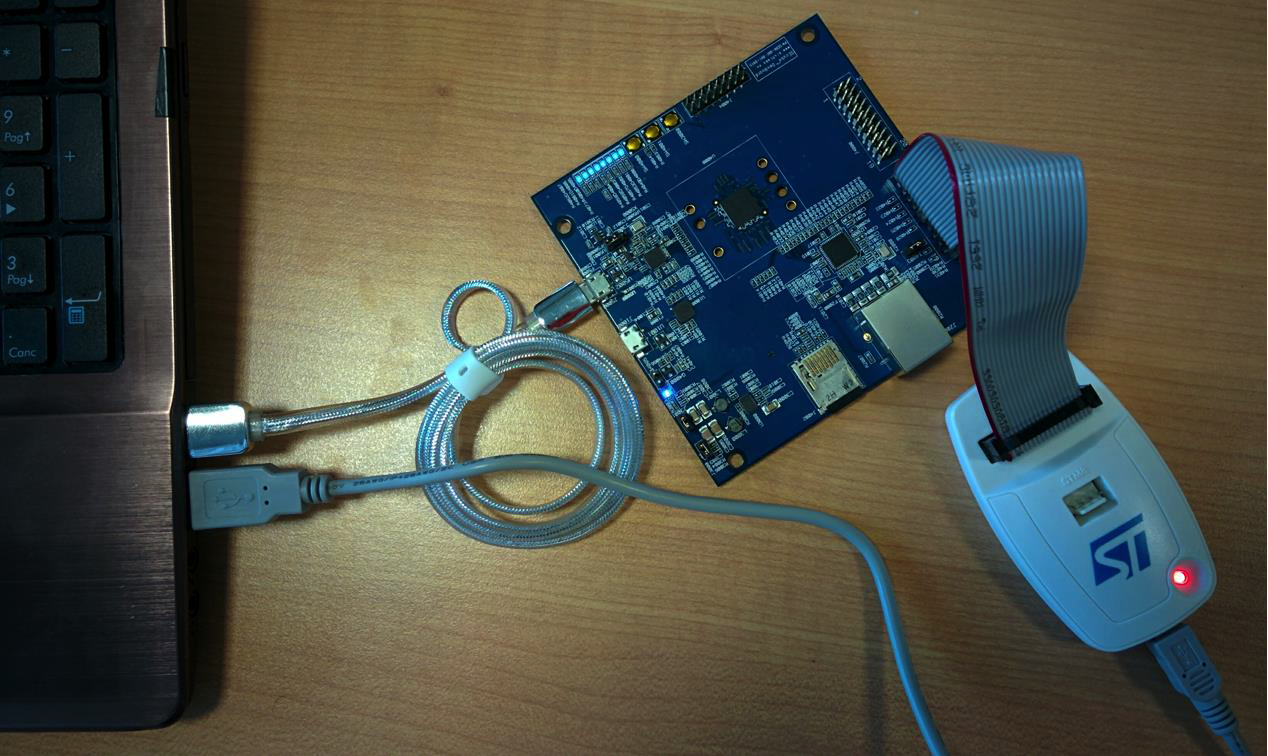
\includegraphics[width=0.42\linewidth]{images/firmware/setup_2}
	\caption{Connection between the STLink/v2 programmer and the SEcube DevKit}
	\label{fig:setup2}
\end{figure}

\begin{figure}
	\centering
	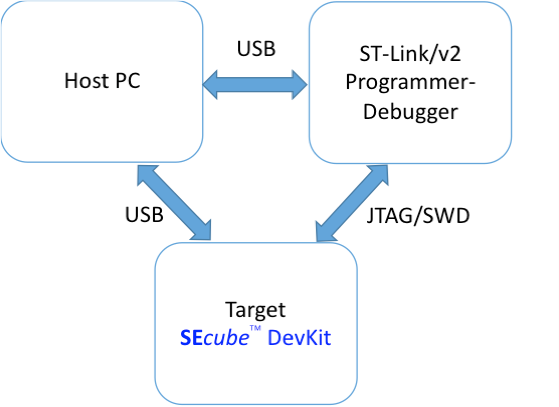
\includegraphics[width=0.35\linewidth]{images/firmware/setup_4}
	\caption{System Architecture}
	\label{fig:setup4}
\end{figure}


Assembling is composed of the following two steps in order to obtain the situation that is available at Figure \ref{fig:setup4}:
\begin{enumerate}
	\item Connect the SEcube DevKit with the programmer by means of the JTAG/SWD cable: the
	cable should be inserted on the JTAG docks on both the programmer (in this case the orientation of the plug is forced from the dock) and the DevKit (in this case you must pay
	attention in inserting the plug on top of both lines of connectors and with its protrusion
	oriented towards the inner side of the DevKit).
	\item Connect the ST-Link/v2 with the PC by means of the USB cable.
\end{enumerate}
The system assembled is shown in Figure \ref{fig:setup2}, while a close-up on the JTAG connection is in Figure \ref{fig:setup3}.

\begin{figure}
	\centering
	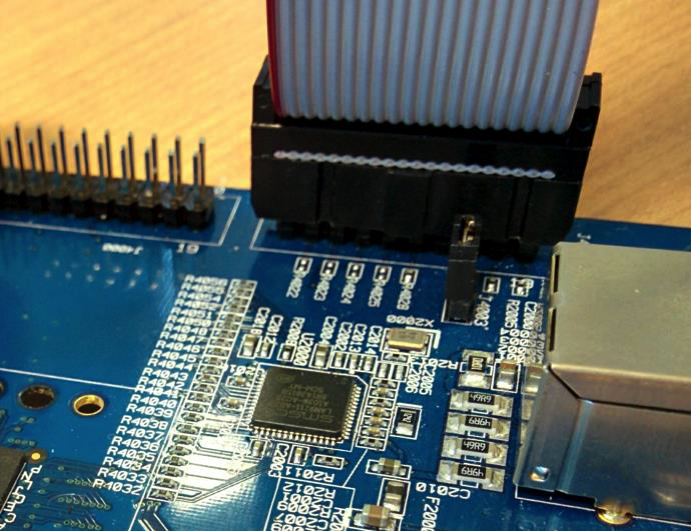
\includegraphics[width=0.35\linewidth]{images/firmware/setup_3}
	\caption{Connection between the STLink/v2 programmer and the SEcubeTM DevKit, close-up (highlighted in red) on the JTAG connector orientation}
	\label{fig:setup3}
\end{figure}


In order to be able to build and flash the firmware, the AC6 Tools must be installed via Eclipse. The AC6 Tool will install the GNU Embedded Toolchain for ARM, which is a ready-to-use, open
source suite of tools for C, C++ and Assembly programming targeting ARM Cortex-M and Cortex-R
family of processors. It includes the GNU Compiler (GCC) and is available free of charge directly
from ARM for embedded so ware development on both Windows and Linux operating systems.
The reference platform for this document is the System Workbench for STM32 (SW4STM32) Eclipse
plugin.

SW4STM32 is an integrated environment that includes:
\begin{itemize}
	\item Building tools (GCC-based ARM cross compiler, assembler and linker);
	\item OpenOCD and GDB debugging tools;
	\item Flash programming tools
\end{itemize}

To install SW4STM32 as an Eclipse plugin:
\begin{enumerate}
	\item launch Eclipse IDE
	\item on the toolbar, click «Help » Install New Software...»
	\item in the Available Software window, click «Add»
	\item in the Add Repository window, set Name and Location fields as follows, and then click «OK»:
	\begin{itemize}
		\item Name: System Workbench for STM32 - Bare Machine edition
		\item Locaton: http://www.ac6-tools.com/Eclipse-updates/org.openstm32.system-workbench.site
	\end{itemize}
	\item select OpenSTM32 Tools and click «Next»
	\item accept the license agreement and click «Finish» to start the plugin installation, continue the installation also if a warning for incompatible or unsigned components is prompted
	\item restart Eclipse
\end{enumerate}



\subsubsection{Firmware flashing}
Once the SECube has been connected to the Host computer via both the ST-Link/v2 programmer and the USB connection, the firmware can be imported, compiled and flashed. 

The latest firmware version has been already compiled and available at ``\textit{SEcube USBStick Firmware/Project/Eclipse/USBStick/Release/USBStick.elf}" but it is possible to import the project into Eclipse and recompile it. If you want to use the pre-compiled version, you can skip the following sections and go to Section \ref{sec:firm_configure}.

In order to import the firmware and the software for performing the init, you need to click «File» and then «Import...», as in Figure \ref{fig:setup6}. At this point after having selected «Existing Projects into Workspace» (Figure \ref{fig:setup7}), the first two projects must be imported (Figure \ref{fig:setup8}).
\begin{figure}[H]
	\centering
	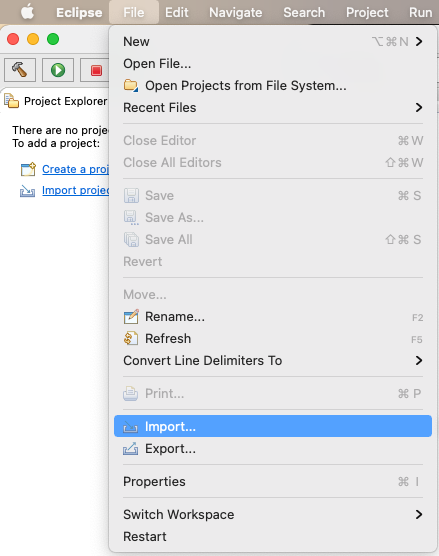
\includegraphics[width=0.35\linewidth]{images/firmware/setup_6}
	\caption{Project import in Eclipse}
	\label{fig:setup6}
\end{figure}
\begin{figure}[H]
	\centering
	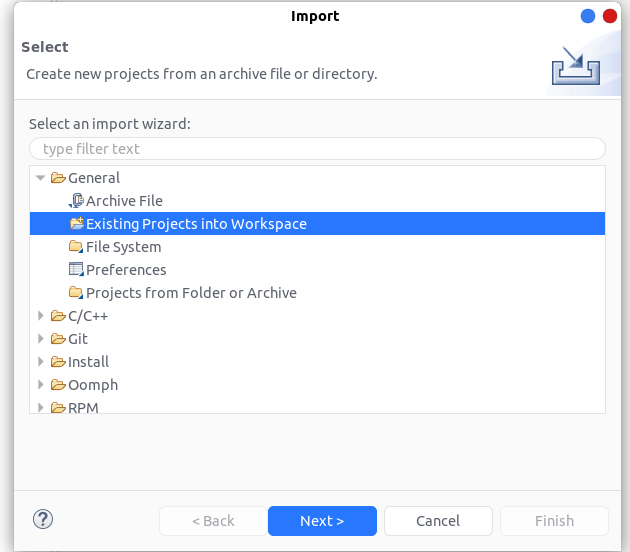
\includegraphics[width=0.55\linewidth]{images/firmware/setup_7}
	\caption{Import of projects}
	\label{fig:setup7}
\end{figure}

\begin{figure}[H]
	\centering
	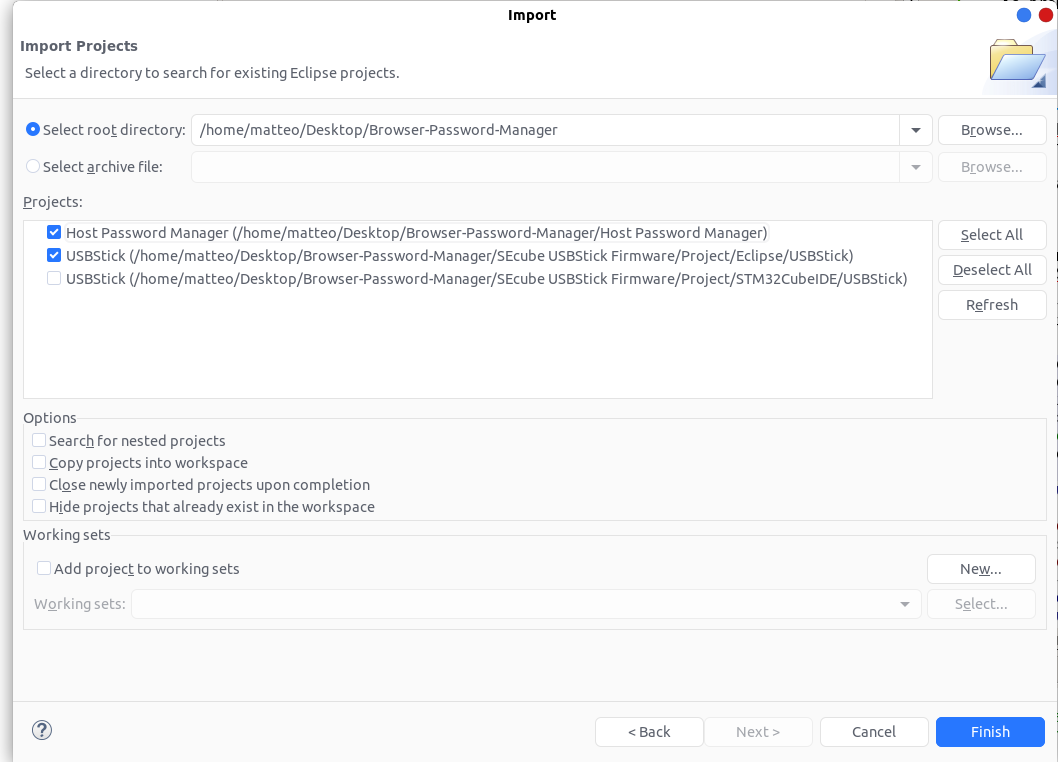
\includegraphics[width=0.55\linewidth]{images/firmware/setup_8}
	\caption{USBStick firmware and Host Password Manager for Initilization}
	\label{fig:setup8}
\end{figure}

The first project will be used during configuration of the device while the second one is the firmware itself.

At this point, on the right you should have two projects, you have to Right click over the ``USBStick" one and select ``Build Project" (refer to Figure \ref{fig:setup10}).
\begin{figure}[H]
	\centering
	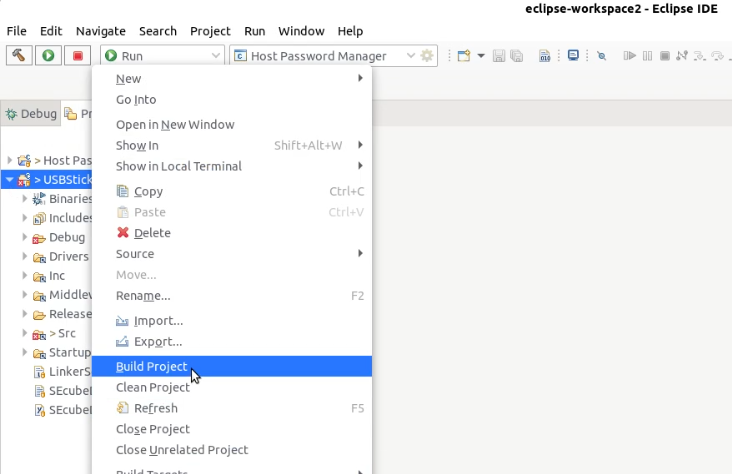
\includegraphics[width=0.55\linewidth]{images/firmware/setup_10}
	\caption{Build the firmware}
	\label{fig:setup10}
\end{figure}

\subsubsection{Configuring the device}
\label{sec:firm_configure}
Once the firmware, you have to first of all to erase the chip in order to remove the previous pin configuration, by doing a Right click on the project and then ``Target" and then ``Erase Chip...". Once it has finished, you can flash the firmware into to the device by clicking ``Target" and then ``Program Chip..." (refer to Figure \ref{fig:setup11}). In the next window you have to select the ``Release" version and flag the ``Reset after program" before clicking ``OK".

\begin{figure}[H]
	\centering
	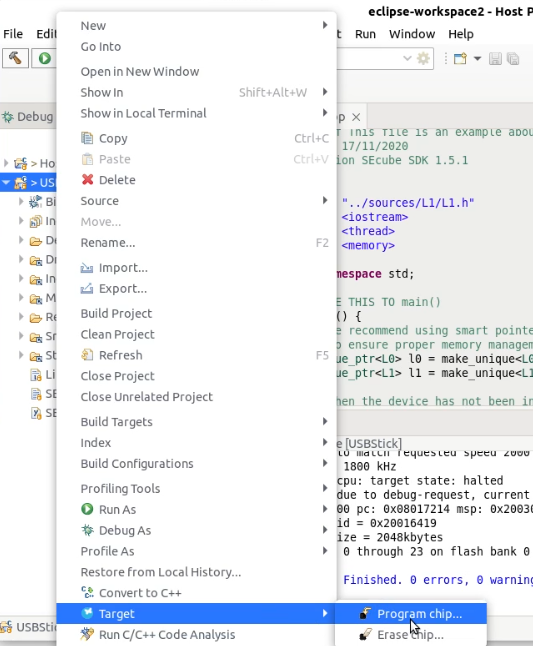
\includegraphics[width=0.55\linewidth]{images/firmware/setup_11}
	\caption{Flash the firmware}
	\label{fig:setup11}
\end{figure}


\begin{figure}[H]
	\centering
	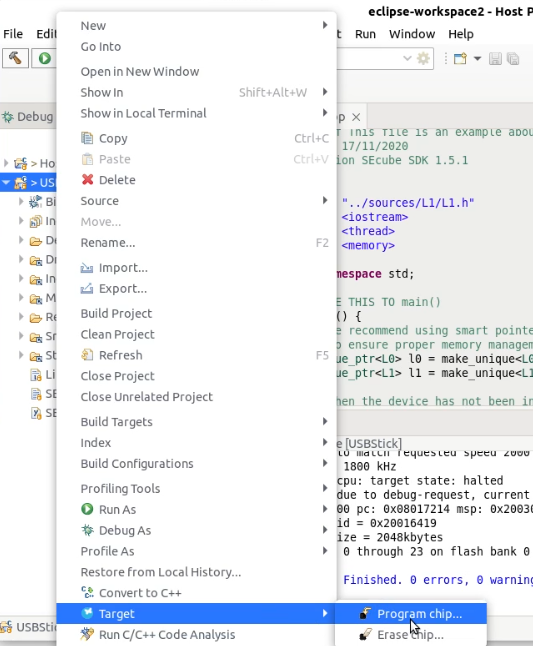
\includegraphics[width=0.55\linewidth]{images/firmware/setup_11}
	\caption{Firmware Release version selection}
	\label{fig:setup12}
\end{figure}

At this point, once the firmware has been flash, you need to configure the device by setting a pin. Now it is the turn of the second project called ``Host Password Manager".\newline\newline
You have to open the \texttt{device\_init.cpp} file and check that the name of the first method is set to \texttt{main}. At this point, you can perform the compilation and run the program. This allows to initialize the device and set the master password for the Secure Password Manager (at line 49 it is possible to change the pin). From now, the device is ready to receive commands by the Host Middleware application in order to manage all passwords features.






